\subsection{Comparing peaks}
\label{sec:AppComparingPeaks}

The processor simulated in Gezel produces the exact same results as our C-code (If we  use $N=32$ in the moving window integration). Assignment 1 specifically asks for $N=30$ in the moving window integration. \\
\\
We tested whether using $N=32$ produced the same peaks in C as $N=30$. For results, see Fig \ref{fig:comparingAllPeaks}.

\begin{figure}[H]
\centering
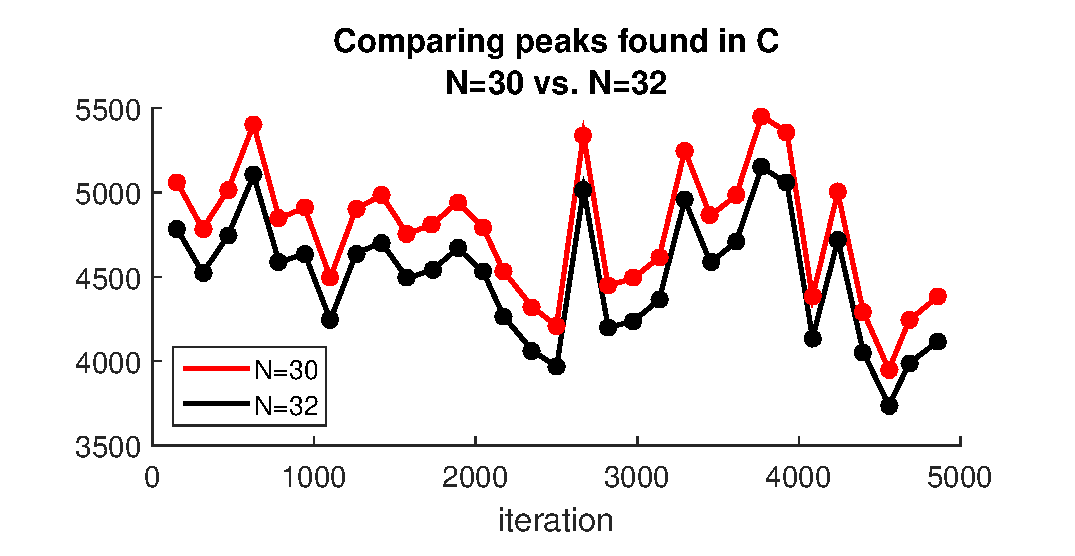
\includegraphics[width=1.0\textwidth]{Appendix/fig/comparingAllPeaks.eps}
\caption{Rpeaks at a given iteration. Using $N=30$ and $N=32$ in C in the moving window integration filter produces similar Rpeaks. Both implementations find 31 Rpeaks at similar iteration steps, i.e. at roughly the same time.}
\label{fig:comparingAllPeaks}
\end{figure}

Both methods identify 31 peaks. The iterations at which peaks are identified differ by an average of $\Delta i = 0.6$, with the most common difference (the mode) being $\Delta i = 0$, i.e. the peaks are found at the same iteration. The peak values are on average $267$ lower using $N=30$, and they are consistently lower, as explained in the Implementation section.